
\documentclass{standalone}
% font set
\usepackage{ctex}
\usepackage{fontspec}
\usepackage[T1]{fontenc}
\usepackage[sc]{mathpazo}
\usepackage{anyfontsize}
\setmainfont{Source Serif 4}
\setsansfont{Source Sans 3}
\setmonofont{Menlo}
\setCJKmainfont[BoldFont=黑体-简 中等,ItalicFont=楷体-简 常规体]{宋体-简 常规体}

% colors
\usepackage[dvipsnames]{xcolor}
\definecolor{pku-red}{RGB}{139,0,18}
\usepackage{colortbl}
\newcommand{\light}[1]{\textcolor{Orchid}{#1}}
\newcommand{\contrastlight}[1]{\textcolor{TealBlue}{#1}}

% plots
\usepackage{tikz}
\usepackage{tikz-cd}
\usetikzlibrary{arrows}
\usetikzlibrary{arrows.meta,positioning,calc,3d}
\usepackage{tikz-3dplot}
\usepackage{pgfplots}
\pgfplotsset{compat=newest}
\tikzset{
    punkt/.style={
        rectangle,
        rounded corners,
        draw=black, very thick,
        minimum height=2em,
        inner sep=6pt,
        text centered,
        fill=gray!30
    }
}

% math package
\let\Bbbk\relax
\usepackage{amsmath}
\usepackage{mathrsfs}
\usepackage{amssymb}
\usepackage{amsfonts}
\usepackage{stmaryrd}
\usepackage{latexsym}
\usepackage{extarrows}
\SetSymbolFont{stmry}{bold}{U}{stmry}{m}{n}


% math notations
\newcommand{\LHS}{\mathrm{LHS}}
\newcommand{\RHS}{\mathrm{RHS}}
\newcommand{\Z}{\mathbb{Z}}
\newcommand{\N}{\mathbb{N}}
\newcommand{\R}{\mathbb{R}}
\newcommand{\Q}{\mathbb{Q}}
\newcommand{\C}{\mathbb{C}}
\newcommand{\E}{\mathbb{E}}
\renewcommand{\O}{\mathcal{O}}
\newcommand{\id}{\mathrm{id}}
\DeclareMathOperator*{\Span}{Span}
\DeclareMathOperator*{\im}{Im}
\DeclareMathOperator*{\rank}{rank}
\DeclareMathOperator*{\card}{card}
\DeclareMathOperator*{\grad}{grad}
\DeclareMathOperator*{\argmax}{argmax}
\DeclareMathOperator*{\epi}{epi}
\DeclareMathOperator*{\maximize}{maximize}
\DeclareMathOperator*{\minimize}{minimize}
\renewcommand{\d}{\mathrm{d}}
\newcommand{\Pow}{\mathcal{P}}
\newcommand{\cov}{\mathsf{Cov}}
\newcommand{\var}{\mathsf{Var}}
\newcommand{\Nor}{\mathcal{N}}
\newcommand{\U}{\mathcal{U}}
\renewcommand{\t}{\mathsf{T}}
\newcommand{\T}{\top}
\newcommand{\F}{\bot}
\newcommand{\norm}[1]{\left\|#1\right\|}
\newcommand{\inner}[2]{\left\langle{#1},{#2}\right\rangle}
\newcommand{\e}{\mathrm{e}}
\newcommand{\const}{\mathrm{const}}
\newcommand{\scB}{\mathscr{B}}
\newcommand{\scF}{\mathscr{F}}
\newcommand{\G}{\mathscr{G}}
\newcommand{\Exp}{\mathsf{Exp}}
\newcommand{\DExp}{\mathsf{DExp}}
\newcommand{\Lap}{\mathsf{Lap}}
\newcommand{\calP}{\mathcal P}
\newcommand{\calS}{\mathcal S}
\newcommand{\calF}{\mathcal F}
\newcommand{\calM}{\mathcal M}
\newcommand{\KL}{\mathrm{KL}}
\newcommand{\ReLU}{\mathsf{ReLU}}
\newcommand{\val}{\mathsf{val}}

\DeclareSymbolFont{symbolsC}{U}{txsyc}{m}{n}
\DeclareMathSymbol{\strictif}{\mathrel}{symbolsC}{74}

\begin{document}
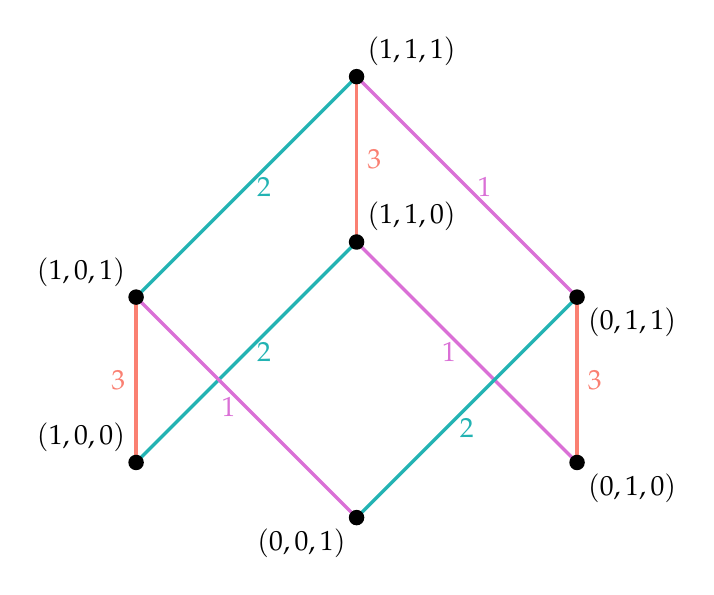
\begin{tikzpicture}[scale=0.7,very thick]
% Coordinates of the vertices
\coordinate (100) at (-4,4);
\coordinate (010) at (4,4);
\coordinate (001) at (0,3);
\coordinate (101) at (-4,7);
\coordinate (110) at (0,8);
\coordinate (011) at (4,7);
\coordinate (111) at (0,11);

% Labels for vertices
\node[above left] at (100) {$(1,0,0)$};
\node[below right] at (010) {$(0,1,0)$};
\node[above right] at (110) {$(1,1,0)$};
\node[below left] at (001) {$(0,0,1)$};
\node[above left] at (101) {$(1,0,1)$};
\node[below right] at (011) {$(0,1,1)$};
\node[above right] at (111) {$(1,1,1)$};

% Draw edges
\draw[TealBlue] (100) -- (110) node[midway,right] {2};
\draw[Salmon] (100) -- (101) node[midway,left] {3};

\draw[Orchid] (010) -- (110) node[midway,left] {1};
\draw[Salmon] (010) -- (011) node[midway,right] {3};

\draw[Orchid] (001) -- (101) node[midway,left] {1};
\draw[TealBlue] (001) -- (011) node[midway,below] {2};

\draw[Salmon] (110) -- (111) node[midway,right] {3};
\draw[TealBlue] (101) -- (111) node[midway,right] {2};
\draw[Orchid] (011) -- (111) node[midway,right] {1};

% Draw vertices as small circles
\foreach \point in {(100), (010), (001), (101), (110), (011), (111)}{
    \fill \point circle (4pt);
}

\end{tikzpicture}
\end{document}
